\documentclass[]{article}
\usepackage[utf8]{inputenc}
\usepackage[top=3cm, bottom=3cm, left=2cm, right=2cm]{geometry}

\usepackage{amsmath}
\usepackage{graphicx}
\graphicspath{{img/}}
\usepackage{wrapfig}
\usepackage{braket}
\usepackage{multicol}

\title{Scintillating Counter of Uranium and Thorium (SCOUT)}
\author{Morgan Askins}
\date{Updated: \today}

\begin{document}
\maketitle
\begin{center}    
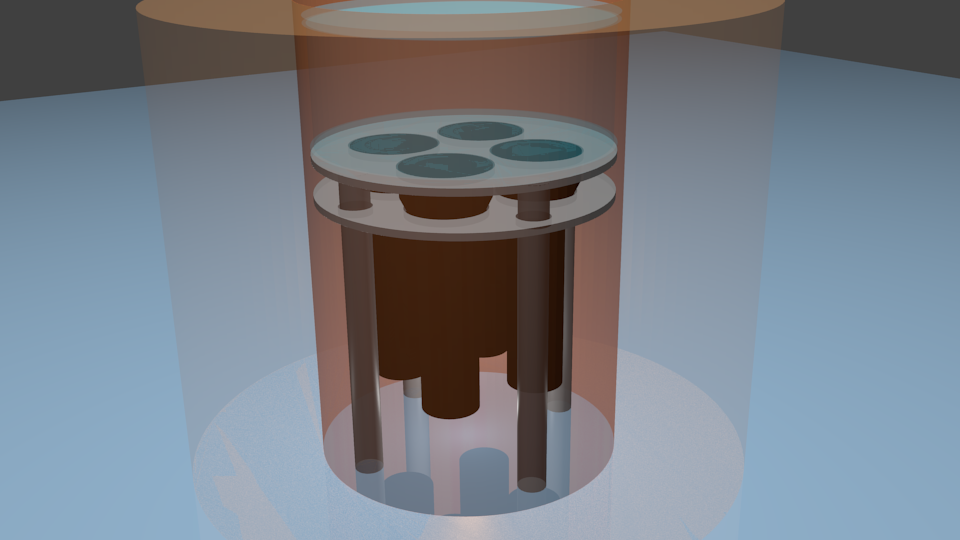
\includegraphics[width=0.8\linewidth]{scout_render.png}
\end{center}
\section{Introduction}
\begin{wrapfigure}{r}{0.25\textwidth}
  \centering
  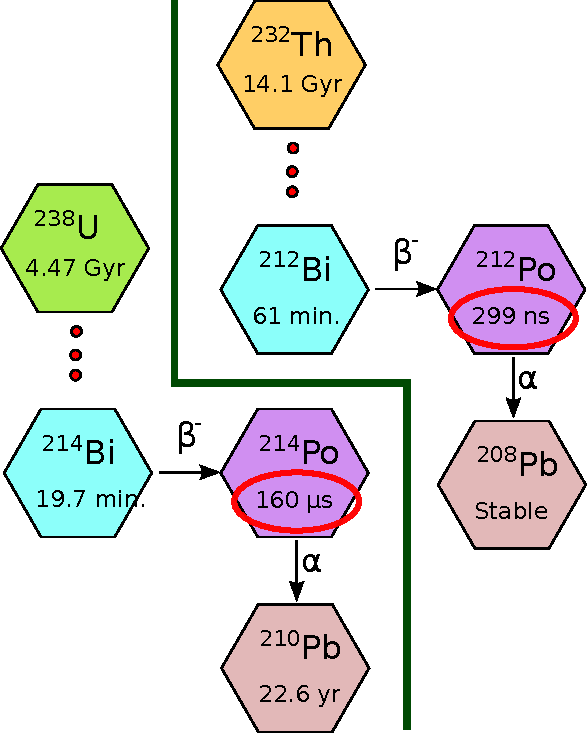
\includegraphics[width=0.25\textwidth]{DecayChain.pdf}
\end{wrapfigure}
Scout is an alpha beta coincidence counter designed to assess the radiopurity of the SNO+
liquid scintillator (Linear Alkylbenzene + 2 g/L 2,5 diphenyloxazole) that arrives
at the surface transfer facility at Snolab. By counting the decays of 
$^{214}Bi\rightarrow^{214}Po\rightarrow^{210}Pb$ in the Uranium decay chain and 
$^{212}Bi\rightarrow^{212}Po\rightarrow^{208}Pb$ in the Thorium decay chain, the
radiopurity can be determined. The expected sensitivity for each of these is of
order $10^{-10}$ g/g for a 24 hour measurement.

\section{Design}
The design for Scout consists of a lead shield from a previous Germanium counter at
UCDavis roughly 4.5" thick. The shield is copper lined on the inside. The inner vessel
is made of acrylic with UV-Transparent acrylic used for the bottom portion which is
coupled to the PMTs. The vessel holds roughly 5 liters of fluid in a short, but wide
cylindrical volume.
Room is left at the bottom for high voltage and signal cables to run from the voltage
dividers out the hole in the bottom to the DAQ. Room is left at the top to
accommodate quick-connect ports for gas and liquid exchange.
\begin{center}
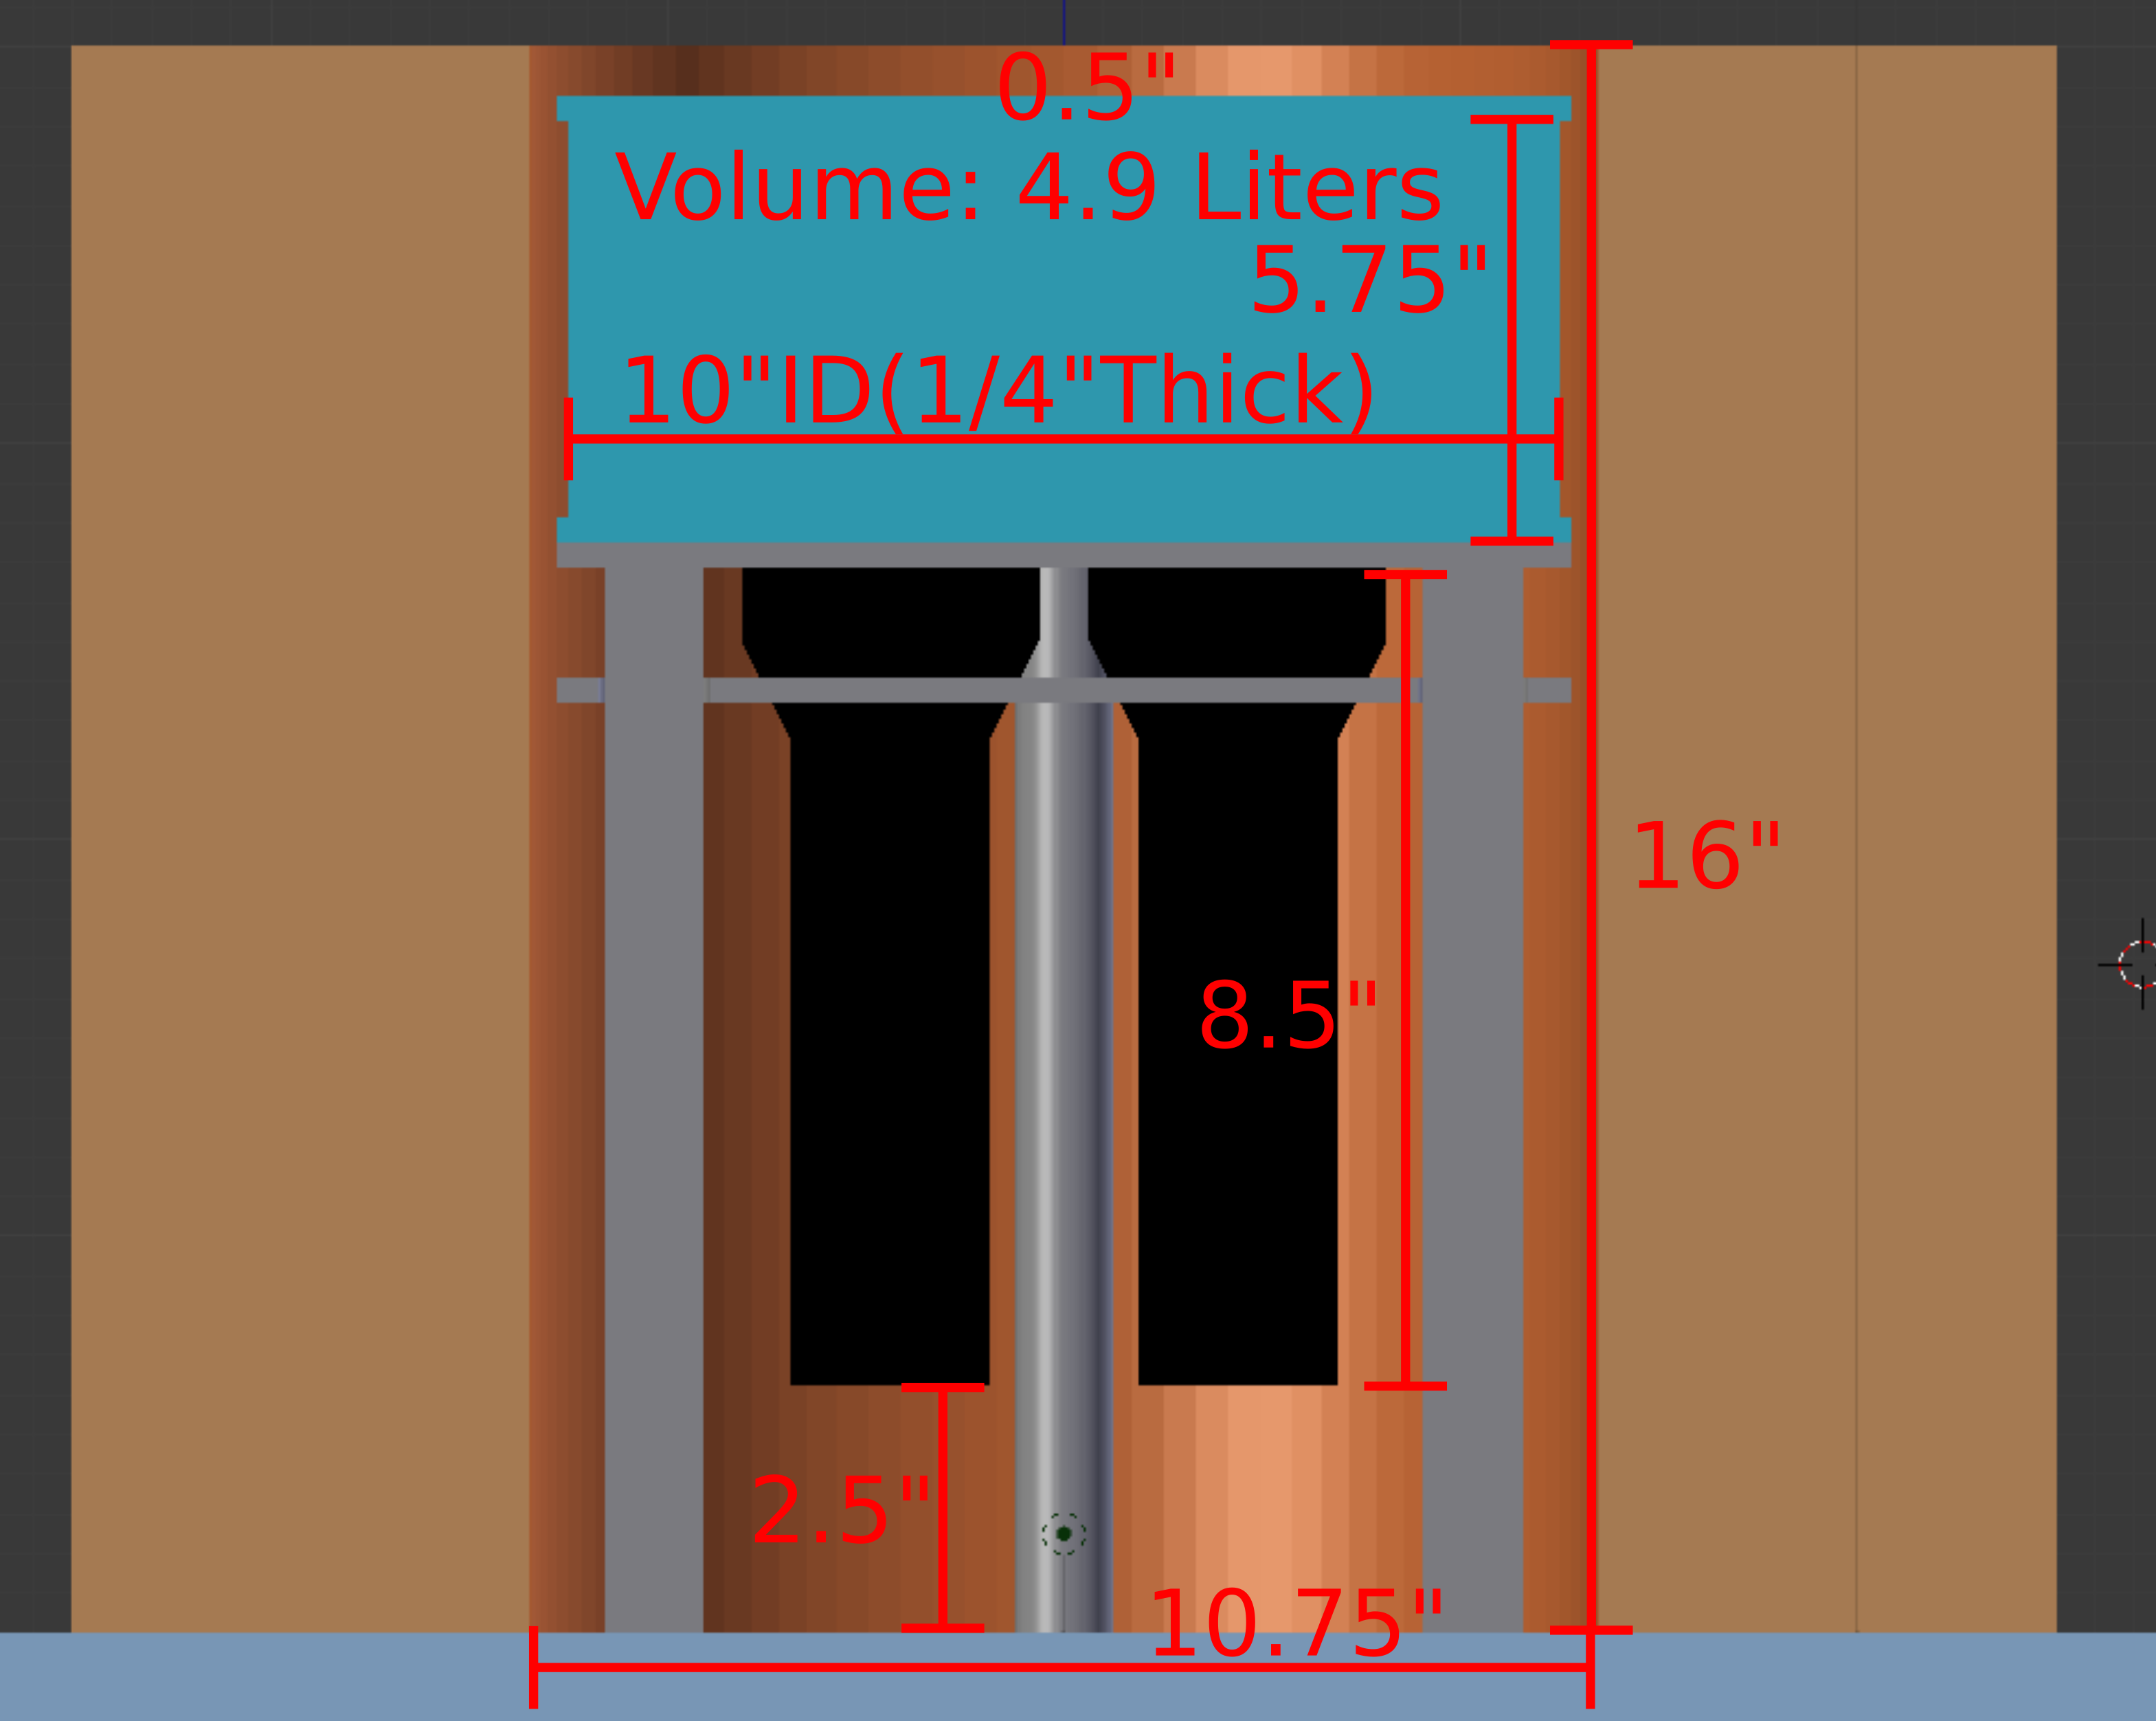
\includegraphics[width=0.5\textwidth]{flat_scout.png}
\end{center}

\section{Data Acquisition}
The four photomultipliers are powered by a desktop CAEN high voltage power supply. The supply
has four channels, so the voltage can be individually adjusted for proper gain matching. The
voltage dividers are negative with a BNC and SHV connector coming directly from them. The BNC
will convert to LIMO and plug into the 16-channel SIS3316 250MHz ADC where only four channels
will be used. The trigger scheme in software can either be set to sum the four channels or
trigger on individual channels. There is not currently a way to require two channels to go
above threshold, but this may be looked into in the future. The coincidence trigger will be
done offline using timing and energy cuts.

\section{Sensitivity}
With the assumption that the LAB is clean to begin with, limtis will be set based on the background
rates, detector volume, and live time. The coincidence window for Bi-Po will help to reject most single
events except those that fall in the same random coincidence window. Based on the energy resolution
of the final design, an energy cut can help to further reduce the background event rate. For a detector
volume of about 5 liters, the sensitivity for a 1 hour run would be about $10^{-10}$ g/g for each
isotope, with $^{238}$U having a slightly better result due to the shorter half-life.

\section{Procedure}
\begin{enumerate}
  \item Assuming we use 5 liters of LAB, measure out PPO at 2g/L (10 grams total) into the
    mixing vessel.
  \item Seal the mixing vessel and connect the nitrogen supply line to the vessel.
  \item Set the pressure just above atmosphere and open the fluid exit port slightly.
  \item Close the fluid exit port, then turn off and disconnect the nitrogen supply.
  \item Fill the mixing vessel with 5 liters of LAB, keeping track of the mass of LAB
    added on a scale.
  \item Place the mixing vessel on the magnetic stirrer for 5 minutes (bar should be in
    there from the start).
  \item While the PPO mixes, prepare the measurement vessel as follows.
  \item Seal the vessel and connect the nitrogen supply line.
  \item Turn off and disconnect the nitrogen supply. This time keep both hoses attached
    and filled with nitrogen.
  \item Quick-connect the hoses to the exchange vessel, then open all valves.
  \item Tilt the vessel in such a way that fluid flows freely through the fluid port,
    and gas flows freely through the gas port.
  \item Close and disconnect the fluid and gas lines.
  \item Begin data acquisition (procedure to be written).
  \item Once DAQ is finished, connect fluid hose to the drain port of the measurement vessel
  \item Open both gas ports to the atmosphere and drain the vessel.
  \item Close and disconnect all hoses.
  \item Empty the mixing vessel into the waste drum.
  \item Clean the hoses and mixing vessel.
  \item {[}It may be possible to clean the AV by filling and rinsing with UPW or LAB{]}
\end{enumerate}

\section{Component List}
\begin{itemize}
  \item 1 metric tonne lead shield on Stand: 2'x2'x5' tall
  \item Waste drum (55 Gallon)
  \item Acrylic Measurement Vessel (~ 5 liters)
  \item Acrylic mobile mixing vessel
  \item Fluid transfer hose with hand valves on both ends
  \item Gas transfer hose with hand valves on both ends
  \item 4x3" Photomultipliers
  \item Desktop High Voltage Supply (Caen)
  \item VME Crate
  \item VME Waveform Digitizer (sis3316 ADC)
  \item VME USB interface (sis3150)
  \item Intel NUC for data recording
  \item External backup storage
  \item Magnetic Stirrer
  \item Chemical Spill Kit
  \item Tubing to connect
\end{itemize}

\end{document}
